\section{Summary diagram}

\begin{figure}[!htb]
    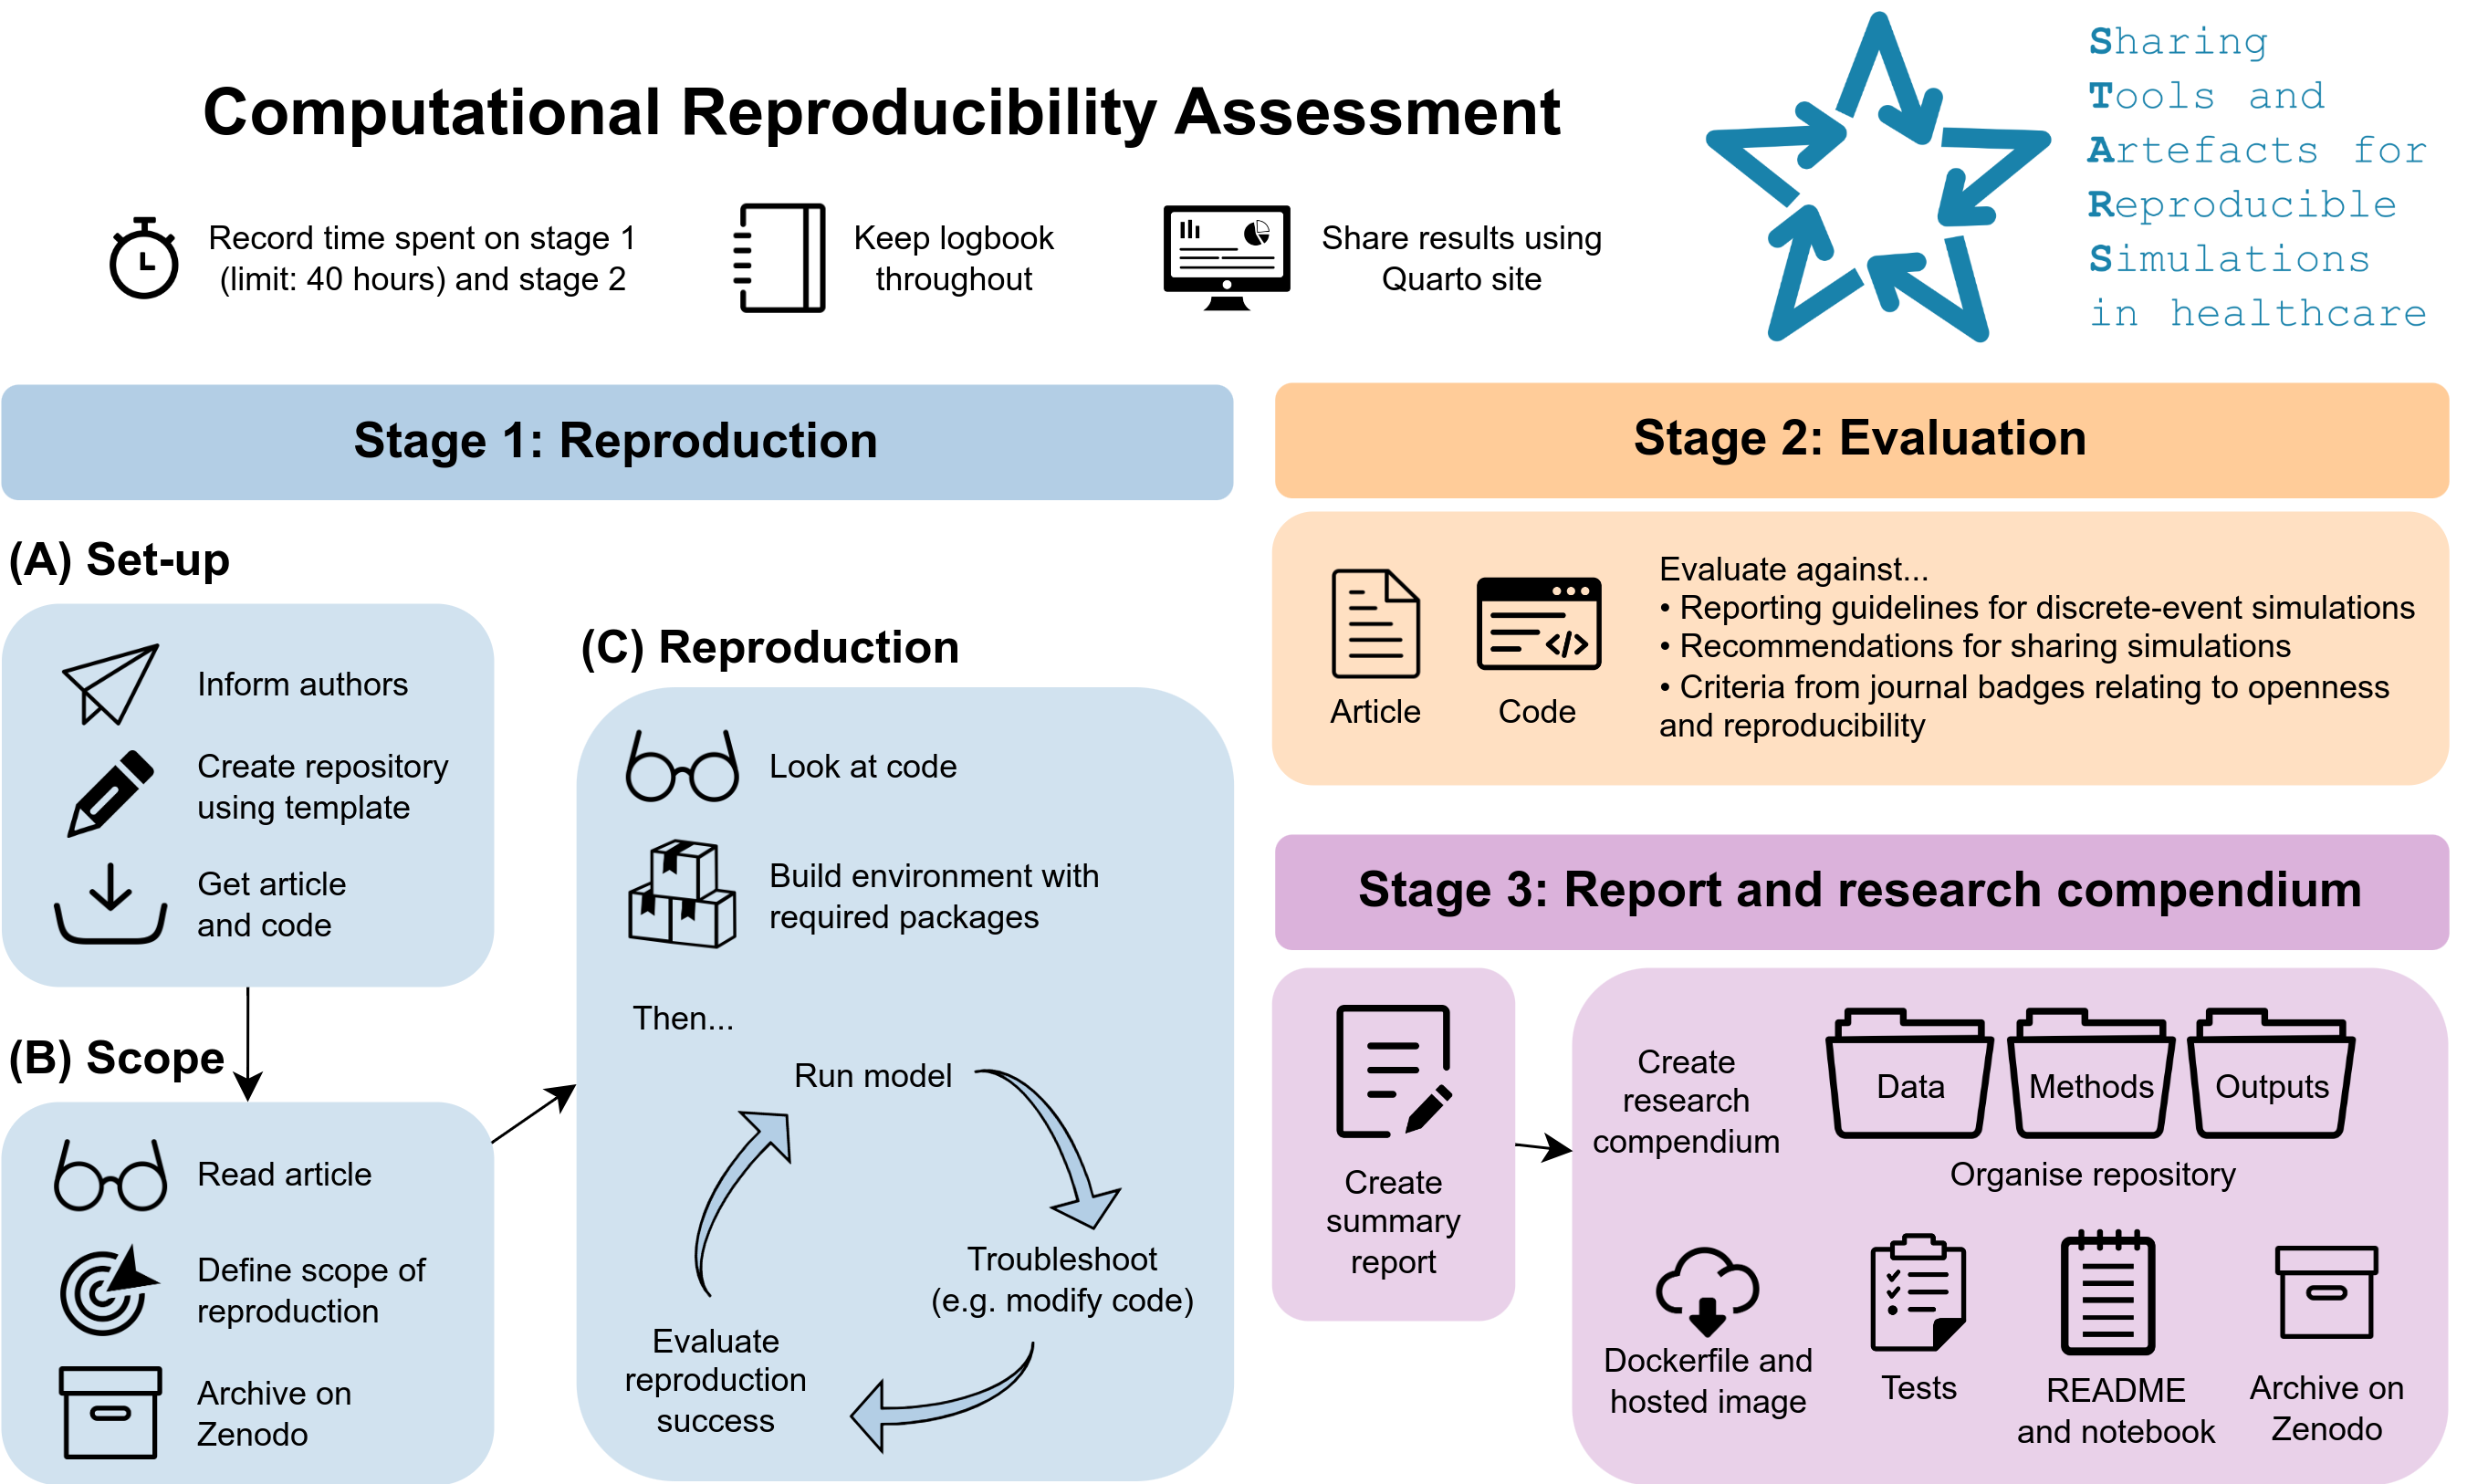
\includegraphics[width=1\linewidth]{images/stars_wp1_workflow.png}
    \caption{Workflow for assessing the computational reproducibility of discrete-event simulation models on STARS.}
    \label{fig:summary}
\end{figure}

\vspace{1cm}
\section{Prerequisites}

This protocol (``Protocol for assessing the computational reproducibility of discrete-event simulation models on STARS") is shared under a CC BY 4.0 license (\url{https://creativecommons.org/licenses/by/4.0/deed.en}). It can be freely used and adapted (with attribution). Please be aware of the following prerequisites:

\begin{itemize}
    \item Python\autocite{python_core_team_python_2024} including typical methods for environment management like conda\autocite{conda_contributors_conda_2023} and virtualenv\autocite{python_packaging_authority_virtualenv_2023}
    \item R\autocite{r_core_team_r_2024} including typical methods for environment management like renv\autocite{ushey_renv_2024}
    \item Quarto\autocite{allaire_quarto_2024}
    \item Docker\autocite{merkel_docker_2014}
    \item GitHub (\url{https://github.com/})
\end{itemize}

\vspace{1cm}
\section{Introduction}

\subsection{Computational reproducibility}

This protocol is focused on \textbf{computational reproducibility}, which is defined as the ability to get consistent results with a prior study when using  the same data and methods as that study.\autocite{national_academies_of_sciences_engineering_and_medicine_reproducibility_2019} Several prior studies assessing computational reproducibility have been used to support and guide development of this protocol:

\begin{itemize}
    \item Krafczyk et al. (2021):\autocite{krafczyk_learning_2021} Assessed the reproducibility of seven articles published in the Journal of Computational Physics.
    \item Wood et al. (2018):\autocite{wood_push_2018,wood_replication_2018} Assessed the reproducibility of 109 published impact evaluations in low- and middle-income countries. Conducted in association with the replication programme of the International Initiative for Impact Evaluation (3ie).
    \item Schwander et al. (2021):\autocite{schwander_replication_2021} Assessed the reproducibility of four health economic obesity models.
    \item Laurinavichyute et al. (2022):\autocite{laurinavichyute_share_2022} Assessed the reproducibility of 118 articles published in the Journal of Memory and Language.
    \item Konkol et al. (2019):\autocite{konkol_computational_2019} Assessed the reproducibility of 41 geoscientific articles from Copernicus Publications and the Journal of Statistical Software
\end{itemize}

It was also guided by:

\begin{itemize}
    \item Ayllón et al. (2021):\autocite{ayllon_keeping_2021} Article with recommendations on keeping modelling notebooks to support completion of TRACE (TRAnsparent and Comprehensive model Evaluation) documents.
    \item The ``Guide for Accelerating Computational Reproducibility (ACRe) in the Social Sciences":\autocite{berkeley_initiative_for_transparency_in_the_social_sciences_guide_2022} Guidelines on conducting reproductions of published social science research.
    \item McManus et al. (2019):\autocite{mcmanus_can_2019} Article proposing several possible definitions for success in reproducing or replicating models in health economics.
    \item Marwick et al. (2018):\autocite{marwick_packaging_2018} Article recommending how to structure data analytical work as research compendiums using the R package structure.
\end{itemize}

\vspace{0.5cm}
\subsection{Present study}

This protocol has been developed as part of the project STARS: ``Sharing Tools and Artefacts for Reproducible Simulations in healthcare". It will be used to assess the computational reproducibility of \textbf{six} published healthcare discrete-event simulation (DES) models. These will be selected from the models identified by Monks and Harper (2023).\autocite{monks_computer_2023} The selection criteria are:

\begin{enumerate}
    \item The model code is \textbf{publicly available}
    \item The model is created using \textbf{Python and R}, as these are popular free and open-source software (FOSS) for the development of models like DES.\autocite{monks_computer_2023} If possible, we will choose an equal split of three Python and three R models.
    \item The code has an \textbf{open license} (either already published, or added upon request from the STARS team).
\end{enumerate}

Throughout the study, results will be openly available and shared via a \textbf{Quarto website}\autocite{allaire_quarto_2024}. This will compile information on the reproduction of the article. This includes the notebooks (.ipynb or .Rmd) producing the items in the scope, as well as a chronological log of work using Quarto blog posts, and then later, the summary report and detailed study results. The protocol will often refer to our \textbf{template repository} which can be viewed here -\url{https://github.com/pythonhealthdatascience/stars_reproduction_template}.\hl{Change to link to Zenodo before publishing}

As in Figure \ref{fig:summary}, there are \textbf{three key stages} to this protocol which should be \textbf{worked through in the following order}:
\begin{enumerate}
    \item Reproduction
    \item Evaluation
    \item Report and research compendium
\end{enumerate}

Two important processes that will need to be \textbf{completed during some or all of the stages} are:
\begin{itemize}
    \item Keeping a detailed record of work using a \textbf{logbook}
    \item \textbf{Timing} how long tasks take to complete
\end{itemize}

\vspace{1cm}
\section{Logbook}

A \textbf{logbook} should be kept throughout \textbf{all three stages} below. It provides a detailed record of work, recorded via \textbf{Quarto blog posts} using the template provided.

As in the guidelines for keeping modelling notebooks from Ayllón et al. (2021),\autocite{ayllon_keeping_2021} the logbooks will consist of \textbf{daily}, dated, chronological entries. \textbf{Tags} will be used to help indicate the activity on each day, and enable posts to be filtered by activity.\autocite{ayllon_keeping_2021} Keeping a detailed log will support later understanding of what was done, and support preparation of final documents like the summary report.

Each entry in the logbook should contain the:
\begin{itemize}
    \item \textbf{Researcher name} and \textbf{date}
    \item \textbf{Tags} (e.g. setup, scope, read, reproduce, guidelines, compendium, report)
    \item \textbf{Time} spent on tasks (if applicable)
    \item \textbf{Comprehensive} record of work. This should include record of working through each stage in the protocol, detailing \textbf{successes} and any \textbf{issues} faced, any \textbf{solutions} found to problems, and any \textbf{changes made to the model code} (noting where and how the code was changed).
    \item Clear statement if and when each item in the scope is considered to have been \textbf{successfully reproduced}.
\end{itemize}

\vspace{1cm}
\section{Timing} \label{sec:timing}

During the first and second stages of the study (\textbf{reproduction} and \textbf{evaluation}) we \textbf{time how long each task takes}. Whilst timing, it is important for the researcher to timestamp when they have:
\begin{itemize}
    \item Finished reproducing each of the items in the scope
    \item Finished working on evaluation of artefacts (badges and recommendations on sharing)
    \item Finished working on evaluation of the article (reporting guidelines)
\end{itemize}

These times should be recorded within the logbook alongside each activity (e.g. 12:10 to 12:45). The times should be monitored with a \textbf{maximum of forty hours} allowed for the first stage (attempting to reproduce the study), as in Krafczyk et al. (2021).\autocite{krafczyk_learning_2021} This cut-off is implemented as we anticipate there would be little more to learn from spending longer than that time on reproducing a single study.

The only exceptions to this timing are:
\begin{itemize}
    \item \textbf{Computation time}. This is at the researcher's discretion. For example, we suggest including short run times during which the researcher is continuously working on the study. However, we would suggest excluding longer run times during which the researcher is no longer working (such as setting the simulation to run for five minutes whilst they make a cup of tea).
    \item \textbf{Time spent by other researchers}. The recorded time should include time spent by the primary researcher on completing tasks, and time spent in discussion with other researchers. However, if other researchers spend time preparing for those discussions (for example, reading the article or looking over the work), this does not need to be included.
\end{itemize}